Impedance measurements of a liquid media can be achieved with different configuration for the electrodes, termed two-, three-, and four-electrodes mode. The most basic one of them is the two-electrode implementation, which uses only two electrodes to apply the electrical stimulus and to measure its response. The signal is provided by the Working Electrode (WE) to the Counter Electrode (CE) \cite{Grossi2017} and is measured between these same two electrodes. The applied signal at the immerged electrodes creates a response in the Sample Under Test (SUT) as well as in both electrolyte-electrode interfaces. This means that the measured response is in fact not only the result of the applied signal on the analyte, but also of the two interfaces’ reactions. These are caused by the polarization of the analyte’s molecules at the interfaces in response to the difference in voltage at the junction. This effect is well-known in surface theory and is called the Electrical Double-Layer (EDL) \cite{grahame1947electrical}. \par
\begin{figure}[h]
    \centering
    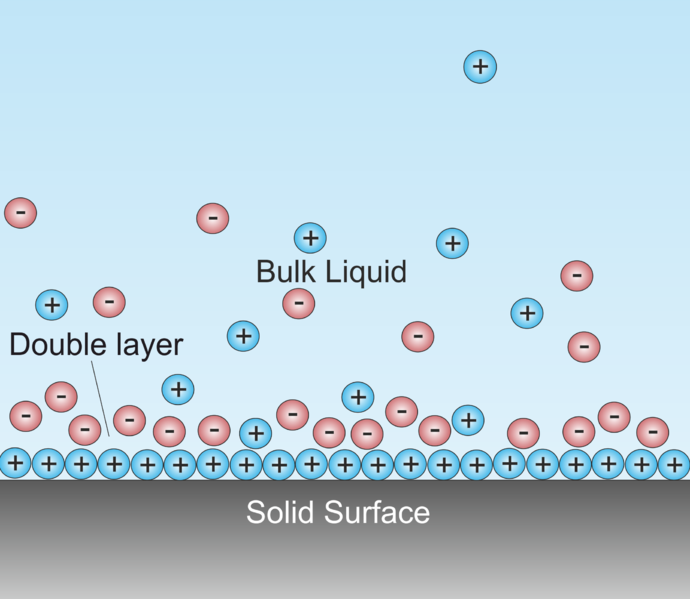
\includegraphics[width=0.6\textwidth]{EDL_image}
    \caption{Schematical view of the behavior of the charged particles at the interface between a charged conductor and an acqueous solution which forms an EDL. \citep{EDL_image}}
    \label{fig:EDL_image}
\end{figure}
The applied signal at the WE causes the electrode’s electrons to accumulate at the electrode’s boundary, as shown in \autoref{fig:EDL_image}, which induces a voltage at the electrode-electrolyte interfaces. This difference in tension causes the electrolyte’s free-moving ions to move toward the junctions, which ultimately result in ions adhering to the electrodes through chemical interactions. These adsorbed ions constitute the first of the two layers. The remaining ions are loosely attracted by the electrode’s charge via the Coulomb force and constitute the second layer, also called the “diffuse layer” \cite{grahame1947electrical}. This arrangement of charged particles creates an insulating gap which behaves similarly to a dielectric and can thus be modelled as a capacitance $C_{dl}$ in series with a resistance $R_i$.  This capacitance accumulates charges, which modifies the desired response in the case of a two-electrodes configuration. Being only a few Ångströms thick, $C_{dl}$ is usually high, in the order of a few $\mu$F \cite{grahame1947electrical}.

An exhaustive model can be used to represent the complex behavior of free-moving charged particles in the electrolyte. Firstly, the diffusion process of ions in a fluidic analyte causes the appearance of a Warburg Element, which can be approximated at high frequency to a Constant Phase Element (CPE) with a phase of 45° and a magnitude inversely proportional to the square root of the frequency:
\begin{equation}
   Z_W = \frac{A_W}{\sqrt{\omega}} + \frac{A_W}{j \sqrt{\omega}}
\end{equation}
Where $A_W$ is the Warburg coefficient, $\omega$ is the complex frequency and $j$ is the imaginary unit. A charge-transfer complex can be observed at the electrode-electrolyte interface, where kinetic exchanges of electrons create residual currents that alter the measured impedance. This charge transfer can be modelized as a resistance $R_{ct}$ Additionally, the capacitance of the EDL can sometimes be more adequately represented as a CPE \cite{gamryBasicsEIS}, following the equation:
\begin{equation}
   Z_{C_{dl}} = \frac{1}{C_{dl}} (j\omega)^\alpha
\end{equation}
Where $Z_{C-{dl}}$ is the impedance of the EDL and $\alpha$ is a constant between -1 and 1. These parameters can be assimilated to a Randles circuit \cite{Randles1947}, which is an equivalent circuit for electrochemical system made of an active electrolyte resistance $R_s$ in series with the parallel capacitance of the EDL $Z_{C{dl}}$ and series combination of the charge-transfer complex resistance $R_{ct}$ and Warburg Element $Z_W$ \cite{gamryBasicsEIS}. The Randles circuit is illustrated in \autoref{fig:EIS_fullmodel}. \par
\begin{figure}[h]
    \centering
    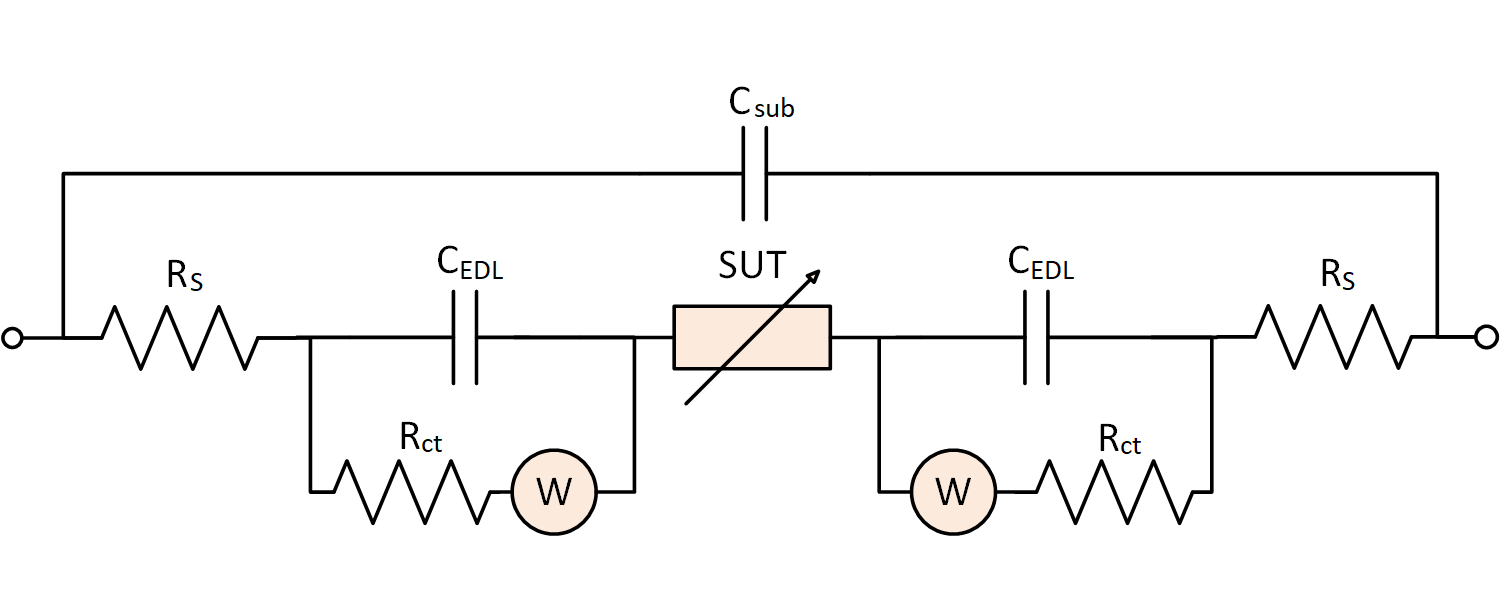
\includegraphics[width=1\textwidth]{EIS_fullmodel}
    \caption{The electrical model of an analyte in an acqueous system sampled using a two-electrode configuration can be defined by two Randles circuit.}
    \label{fig:EIS_fullmodel}
\end{figure}

With the use of electrodes made of inert material such as gold or platinum, it is possible to reduce the effect of the charge-transfer complex. It is also possible to neglect the effect of the Warburg Element with an adequate selection of the measurement frequencies since the Warburg impedance mostly affects the results at low frequency. That lower bound for the frequency depends mostly on the type and shape of the electrodes \cite{Randles1947}. With these precautions taken, the complex Randles circuit can be simplified to the model presented in \autoref{fig:EIS_simplemodel} It is important to remember that those models only superficially describe the true complex dielectric behavior seen in microfluidics for real biological cells and microparticles \cite{Gawad2004}, and that extracting the numerical values associated to these model poses quite a challenge in practice (refer to \autoref{sec:CellModel} and \autoref{sec:IFC}). \par
\begin{figure}[h]
    \centering
    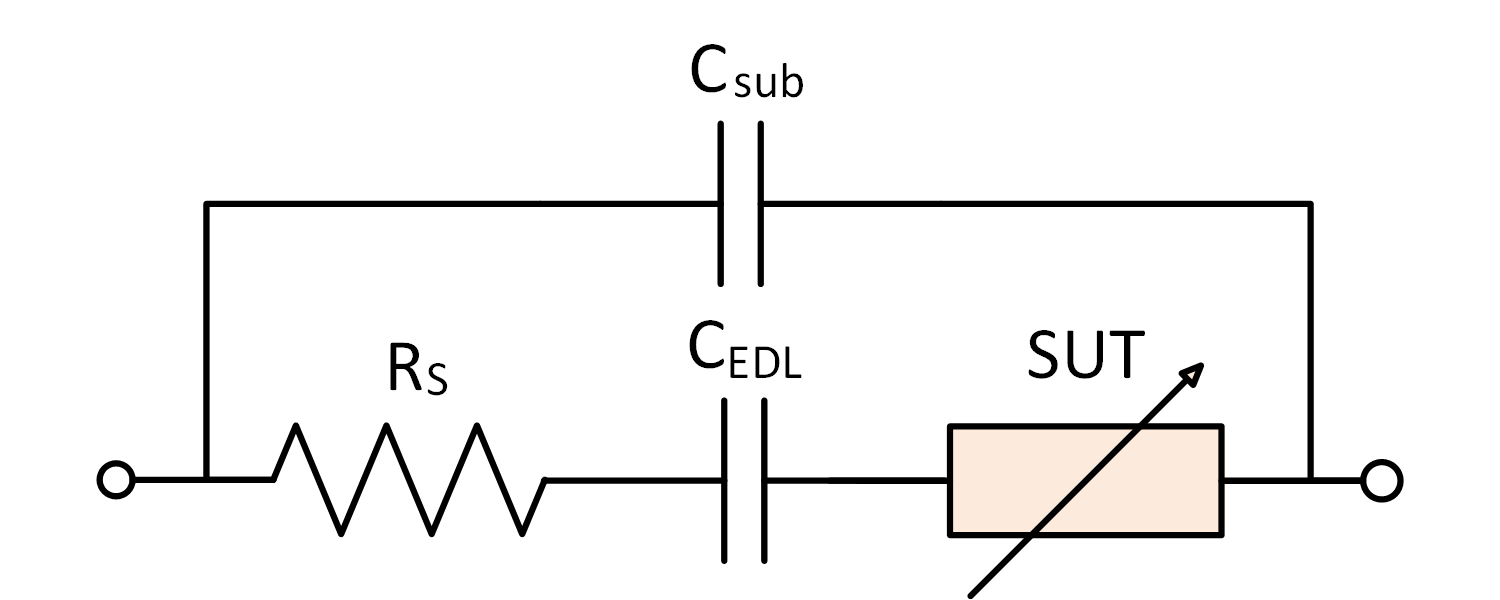
\includegraphics[width=0.7\textwidth]{EIS_simplemodel}
    \caption{The simplified electrical model of an analyte in an acqueous system sampled using a two-electrodes configuration.}
    \label{fig:EIS_simplemodel}
\end{figure}

Three-electrodes configuration uses another electrode, the Reference Electrode (RE), in order to provide a tension reference for the applied signal that is independent of the measured signal. The measurement is in this way partially dissociated from the applied signal: the measured impedance now considering only the response of the SUT and of the WE-electrolyte interface. The three-electrodes configuration offers better performance than its two-electrodes counterpart since the kinetical electrodes’ polarization is mostly an asymmetrical reaction: the charge transfer and diffusion happening at the WE are different than those happening at the CE since the difference in potential is different at the two junctions. Therefore, considering only the influence of the WE on the measured impedance gives better consistency on the results \cite{Grossi2017}. \par

Another electrode, the Working Sensing Electrode (WSE), can be added to obtain the four-electrodes configuration. In this mode, the applied signal is produced at the WE and CE and the measured signal is taken at the WSE and RE. By so doing, the measured impedance is completely dissociated of the interfaces’ behaviors since no current is drawn at either junction \cite{Grossi2017}. Using a higher number of electrodes gives more precise results at the price of complexity; thus, the choice of the number of electrodes depends on the specific application. It must also be mentioned that in some applications, the response of the interfaces can yield results just as important as the response of the electrolyte, the two- and three-electrode configurations should then not be discarded too hastily. \par

Interdigitated electrodes (IDEs) can also be used for impedance measurements. They show great promise because of their low ohmic drop, excellent signal to noise ration, robustness, and high sensitivity. They also do not need a reference electrode, which makes for a simpler implementation in a limited chip area. They are made from two separate interlocking electrodes, usually made from gold or platinum due to their biocompatibility, and inertness. The detection sensibility is usually a function of the size of the IDEs fingers; choosing smaller fingers results in a higher sensitivity \cite{Khormazard2016}.  \par
\begin{figure}[h]
    \centering
    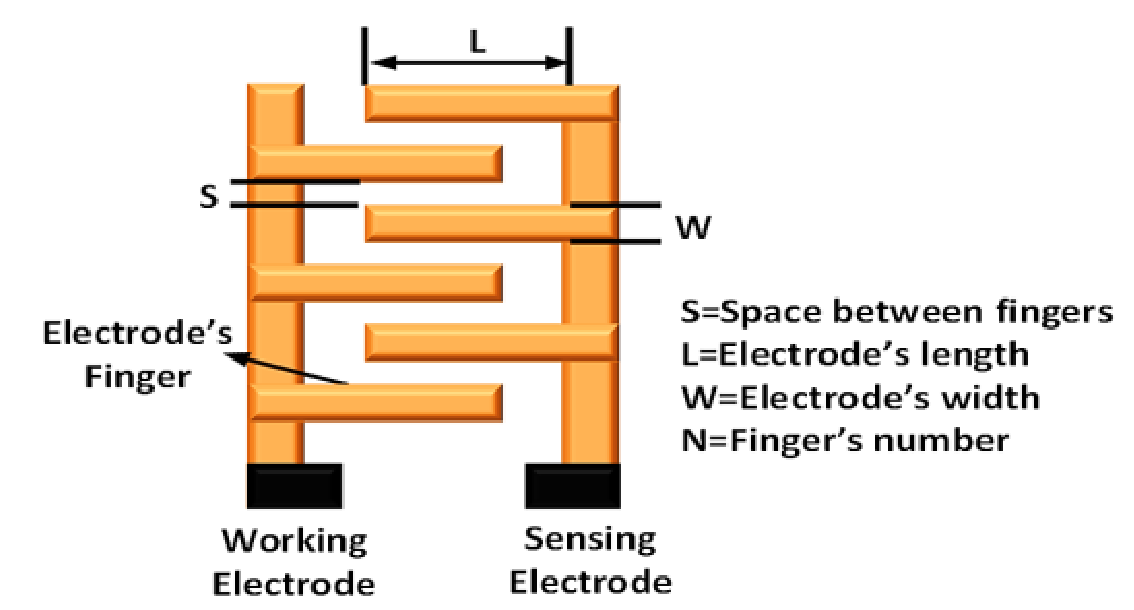
\includegraphics[width=0.8\textwidth]{Nazilah_IDE}
    \caption{Interdigitated electrodes \citep{hosseini2021optimization}}
    \label{fig:Nazilah_IDE}
\end{figure}

Faster measurement times can be achieved by using Multi-Electrode Array (MEA): a higher number of electrodes permits parallel measurements, which increase the device’s throughput \cite{Rajabzadeh2019EIS}. However, increasing the number of channels is also associated with increased digital complexity and data rates.